% $Id$
%

\section{Bootstrap}


%%---------------------------------------------------------------

\begin{frame}
\frametitle{�Qu� es Bootstrap?}

\begin{itemize}
  \item Bootstrap es un framework libre para desarrollo web
  \item Realizado por ingenieros de Twitter
  \item Incluye plantillas HTML y CSS con tipograf�as, formas, botones, cuadros, barras de navegaci�n, carruseles de im�genes y muchas otras
  \item Tambi�n existe la posibilidad de utilizar plugins de JavaScript
  \item Aunque su preferencia es \emph{mobile first}, permite crear dise�os que se ven bien en m�ltiples dispositivos (\emph{responsive design})
\end{itemize}

\end{frame}

%%---------------------------------------------------------------

\begin{frame}
\frametitle{Ventajas de Bootstrap (para ingenieros)}

\begin{itemize}
  \item Es sencillo y r�pido
  \item Se adapta a distintos dispositivos (\emph{responsive design})
  \item Proporciona un dise�o consistente
  \item Es compatible con los navegadores modernos
  \item Es software libre
\end{itemize}

\end{frame}

%%---------------------------------------------------------------

\begin{frame}[fragile]
\frametitle{Ficheros de Bootstrap}

\begin{footnotesize}
\begin{verbatim}
bootstrap/
|--- css/
|   |--- bootstrap.css
|   |--- bootstrap.css.map
|   |--- bootstrap.min.css
|   |--- bootstrap-theme.css
|   |--- bootstrap-theme.css.map
|   |--- bootstrap-theme.min.css
|--- js/
|   |--- bootstrap.js
|   |--- bootstrap.min.js
|--- fonts/
    |--- glyphicons-halflings-regular.eot
    |--- glyphicons-halflings-regular.svg
    |--- glyphicons-halflings-regular.ttf
    |--- glyphicons-halflings-regular.woff
    |--- glyphicons-halflings-regular.woff2
\end{verbatim}
\end{footnotesize}

\end{frame}


%%---------------------------------------------------------------

\begin{frame}[fragile]
\frametitle{La plantilla de Bootstrap}


\begin{footnotesize}
\begin{verbatim}
<!DOCTYPE html>
<html>
<head>
  <meta charset="utf-8">
  <title>Basic Bootstrap Template</title>
  <meta name="viewport" content="width=device-width, initial-scale=1.0">
  <link rel="stylesheet" type="text/css" href="css/bootstrap.min.css">
</head>
<body>
  <h1>Hello, world!</h1>
  <script src="http://code.jquery.com/jquery.min.js"></script>
  <script src="js/bootstrap.min.js"></script>
</body>
</html>
\end{verbatim}
\end{footnotesize}

\end{frame}



%%---------------------------------------------------------------

\begin{frame}[fragile]
\frametitle{Bootstrap en CDN}

\begin{itemize}
  \item Con un CDN (Content Delivery Network) no hace falta tener Bootstrap en nuestros
archivos. Adem�s, si un usuario ya ha descargado esas URLs, probablemente
las tenga ya en la cach� del navegador (con el consiguiente ahorro de tiempo).
\end{itemize}

\begin{footnotesize}
\begin{verbatim}
 <!-- Latest compiled and minified CSS -->
<link rel="stylesheet" 
href="http://maxcdn.bootstrapcdn.com/bootstrap/3.2.0/css/bootstrap.min.css">

<!-- jQuery library -->
<script 
 src="https://ajax.googleapis.com/ajax/libs/jquery/1.11.1/jquery.min.js">
</script>

<!-- Latest compiled JavaScript -->
<script 
 src="http://maxcdn.bootstrapcdn.com/bootstrap/3.2.0/js/bootstrap.min.js">
</script>
\end{verbatim}
\end{footnotesize}


\end{frame}


%%---------------------------------------------------------------

\begin{frame}[fragile]
\frametitle{Mobile first}

% Info: https://developer.mozilla.org/es/docs/M%C3%B3vil/Viewport_meta_tag

\begin{itemize}
  \item En los navegadores, el \emph{viewport} es la parte visible de un documento
  \item Si el documento es mayor que el �rea de visualizaci�n, el usuario puede cambiar la vista desplaz�ndose
  \item Con una propiedad de etiqueta meta, podemos indicar la escala inicial del \emph{viewport}
\end{itemize}

\begin{footnotesize}
\begin{verbatim}
<meta name="viewport" content="width=device-width, initial-scale=1">
\end{verbatim}
\end{footnotesize}

\begin{itemize}
  \item Se puede inhabilitar el zoom en dispositivos m�viles con \texttt{user-scalable=no}
  \item Los usuarios s�lo podr�n hacer \emph{scroll} y tendr� una apariencia nativa.
  \item Usar con precauci�n. No vale para todas las aplicaciones
\end{itemize}

\begin{footnotesize}
\begin{verbatim}
<meta name="viewport" content="width=device-width, initial-scale=1, 
maximum-scale=1, user-scalable=no">
\end{verbatim}
\end{footnotesize}

\end{frame}


%%---------------------------------------------------------------

\begin{frame}[fragile]
\frametitle{Contenedores}

\begin{itemize}
   \item Bootstrap requiere tener un elemento contenedor que cubra contenidos y el sistema de rejilla.
   \item Para un contenedor responsivo de tama�o fijo, usa \texttt{.container}
\end{itemize}

\begin{footnotesize}
\begin{verbatim}
<div class="container">
  ...
</div>
\end{verbatim}
\end{footnotesize}

\begin{itemize}
  \item Si se desea un contenedor con el ancho total (del \emph{viewport}), se ha de usar \texttt{.container-fluid}
\end{itemize}

\begin{footnotesize}
\begin{verbatim}
<div class="container-fluid">
  ...
</div>
\end{verbatim}
\end{footnotesize}

\end{frame}



%%---------------------------------------------------------------

\begin{frame}
\frametitle{El sistema de rejilla (I)}

El dise�o de p�ginas basado en rejilla se realiza mediante filas y
columnas donde se colocan los contenidos. As� funciona la rejilla de Bootstrap:

\begin{itemize}

  \item Filas, dentro un contenedor, agrupan horizontalmente varias columnas, que son las que tienen contenido
  \item La pantalla se divide en 12 columnas
  \item Las columnas definen su anchura especificando cu�ntas columnas de la fila ocupan
  \item Hay clases CSS (como por ejemplo .row y .col-xs-4) para crear rejillas r�pidamente
  \item Hay padding entre columnas. En la primera y �ltima columnas, las filas (elementos .row) aplican m�rgenes negativos

\end{itemize}

\end{frame}

%%---------------------------------------------------------------

\begin{frame}[fragile]
\frametitle{El sistema de rejilla (y II)}

% Ejemplos: http://getbootstrap.com/examples/grid/

\begin{center}
\begin{figure}[p]
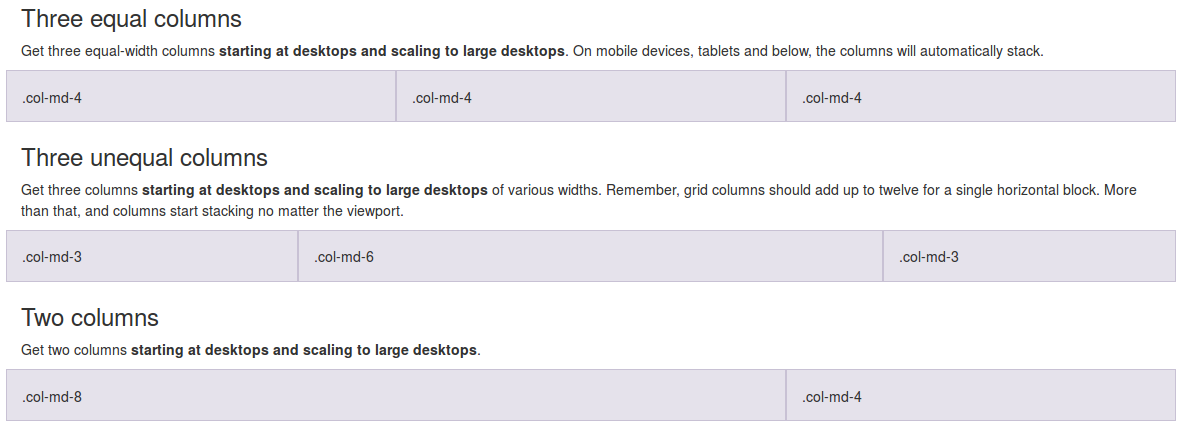
\includegraphics[width=0.99\textwidth]{figs/grid.png}
\end{figure}
\end{center}

\end{frame}



%%---------------------------------------------------------------

\begin{frame}[fragile]
\frametitle{Responsive design}

\begin{center}
\begin{figure}[p]
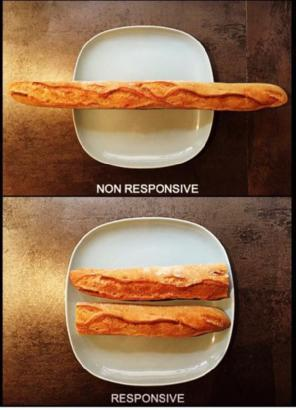
\includegraphics[width=0.99\textwidth]{figs/responsive.jpg}
\end{figure}
\end{center}

\begin{flushright}
{\tiny
Source: https://image-store.slidesharecdn.com/420d15aa-cbf0-4ded-ac42-fcf728610bc1-original.jpeg
}
\end{flushright}

\end{frame}



%%---------------------------------------------------------------

\begin{frame}[fragile]
\frametitle{Responsive design en Bootstrap}

M�viles y escritorio:

\begin{center}
\begin{figure}[p]
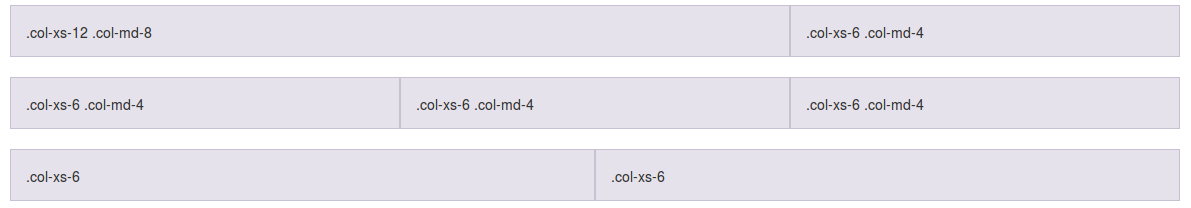
\includegraphics[width=0.99\textwidth]{figs/grid-responsive.png}
\end{figure}
\end{center}

M�vil, tableta y escritorio:

\begin{center}
\begin{figure}[p]
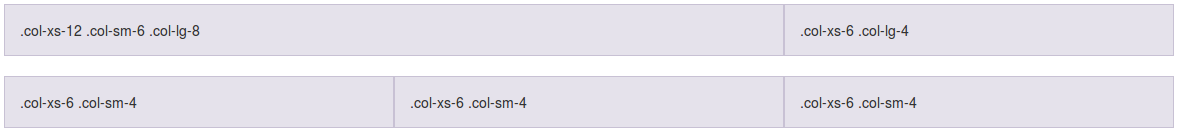
\includegraphics[width=0.99\textwidth]{figs/grid-responsive2.png}
\end{figure}
\end{center}

\end{frame}



%%---------------------------------------------------------------

\begin{frame}[fragile]
\frametitle{Media queries}

Bootstrap utiliza \emph{media queries} para establecer puntos de ruptura en los que la rejilla se transforma para adaptarse a cada dispositivo.

\begin{footnotesize}
\begin{verbatim}
/* Extra small devices (phones, less than 768px) */
/* No media query since this is the default in Bootstrap */

/* Small devices (tablets, 768px and up) */
@media (min-width: @screen-sm-min) { ... }
/* Medium devices (desktops, 992px and up) */
@media (min-width: @screen-md-min) { ... }
/* Large devices (large desktops, 1200px and up) */
@media (min-width: @screen-lg-min) { ... }
\end{verbatim}
\end{footnotesize}


Se pueden utilizar tambi�n \emph{media queries} que definen la propiedad max-width y restringen los dispositivos a los que se aplican los estilos:

\begin{footnotesize}
\begin{verbatim}
@media (max-width: @screen-xs-max) { ... }
@media (min-width: @screen-sm-min) and (max-width: @screen-sm-max) { ... }
@media (min-width: @screen-md-min) and (max-width: @screen-md-max) { ... }
@media (min-width: @screen-lg-min) { ... }
\end{verbatim}
\end{footnotesize}


\end{frame}



%%---------------------------------------------------------------

\begin{frame}
\frametitle{Otras clases}

Bootstrap viene con una serie de estilos (generalmente en formato de clase CSS)
por defecto, entre otros:

\begin{itemize}
  \item \texttt{table}
  \item \texttt{form}
  \item \texttt{buttons}
  \item \texttt{img-responsive}
  \item \texttt{helper} classes
  \item y otras utilidades responsivas
\end{itemize}

\end{frame}


%%---------------------------------------------------------------

\begin{frame}
\frametitle{JavaScript}

Con Bootstrap vienen una serie de \emph{plug-ins} de JavaScript, como:

\begin{itemize}
  \item transitions.js: efectos de transici�n
  \item modal.js: di�logos simples y flexibles
  \item dropdown.js: men�s desplegables
  \item scrollspy.js: seg�n vamos bajando en la p�gina, actualiza la \emph{navbar}
  \item tab.js: pesta�as
  \item tooltip.js y popover.js: cajas con consejos o m�s informaci�n
  \item alert.js: alertas
  \item button.js: botones
  \item collapse.js: permite mostrar/ocultar elementos
  \item carousel.js: el (ya famoso carrusel)
  \item affix.js: Men� de navegaci�n lateral
\end{itemize}

\end{frame}


%%---------------------------------------------------------------

\begin{frame}
\frametitle{Bootlint}

\begin{itemize}
  \item Herramienta que detecta algunos errores comunes el HTML de dise�os \texttt{Bootstrap}
  \item Comprueba que las instancias de componentes Bootstrap han sido correctamente estructurados
  \item Analiza tambi�n la inclusi�n de ciertas etiquetas $<meta>$, la declaraci�n DOCTYPE HTML5, etc.
  \item P�gina web: \url{https://github.com/twbs/bootlint}
\end{itemize}

\end{frame}

%%---------------------------------------------------------------

\begin{frame}
\frametitle{Otros sitios de inter�s}



\begin{itemize}
  \item Listado de recursos sobre Bootstrap \\
        \url{http://bootsnipp.com/resources}
  \item Bootsnipp: Cientos de componentes adicionales \\
        \url{http://www.bootsnipp.com}
  \item Startboostrap: Plantillas y temas Bootstrap (gratis) \\
        \url{http://startbootstrap.com/}  
  \item WrapBoostrap: Plantillas y temas Boostrap (de pago) \\
        \url{https://wrapbootstrap.com/}
  \item BootTheme: Generador (no libre) de dise�os Bootstrap \\
        \url{http://www.boottheme.com/}
\end{itemize}

\end{frame}


